% Тип документа
\documentclass[a4paper,12pt]{extarticle}

% Шрифты, кодировки, символьные таблицы, переносы
\usepackage{cmap}
\usepackage[T2A]{fontenc}
\usepackage[utf8x]{inputenc}
\usepackage[russian]{babel}

% Это пакет -- хитрый пакет, он нужен но не нужен
\usepackage[mode=buildnew]{standalone}

\usepackage
	{
		% Дополнения Американского математического общества (AMS)
		amssymb,
		amsfonts,
		amsmath,
		amsthm,
		physics,
		% misccorr,
		% 
		% Графики и рисунки
		wrapfig,
		graphicx,
		subcaption,
		float,
		tikz,
		tikz-3dplot,
		caption,
		csvsimple,
		color,
		booktabs,
		pgfplots,
		pgfplotstable,
		geometry,
		% 
		% Таблицы, списки
		array,
		makecell,
		multirow,
		indentfirst,
		%
		% Интегралы и прочие обозначения
		ulem,
		esint,
		esdiff,
		% 
		% Колонтитулы
		fancyhdr,
	}  

\usepackage{xcolor}
\usepackage{hyperref}

 % Цвета для гиперссылок
\definecolor{linkcolor}{HTML}{000000} % цвет ссылок
\definecolor{urlcolor}{HTML}{799B03} % цвет гиперссылок
 
\hypersetup{pdfstartview=FitH,  linkcolor=linkcolor,urlcolor=urlcolor, colorlinks=true}
% Обводка текста в TikZ
\usepackage[outline]{contour}

% Увеличенный межстрочный интервал, французские пробелы
\linespread{1.3} 
\frenchspacing 

 
\usetikzlibrary
	{
		decorations.pathreplacing,
		decorations.pathmorphing,
		patterns,
		calc,
		scopes,
		arrows,
		fadings,
		through,
		shapes.misc,
		arrows.meta,
		3d,
		quotes,
		angles,
		babel
	}


\tikzset{
	force/.style=	{
		>=latex,
		draw=blue,
		fill=blue,
				 	}, 
	%				 	
	axis/.style=	{
		densely dashed,
		blue,
		line width=1pt,
		font=\small,
					},
	%
	th/.style=	{
		line width=1pt},
	%
	acceleration/.style={
		>=open triangle 60,
		draw=magenta,
		fill=magenta,
					},
	%
	inforce/.style=	{
		force,
		double equal sign distance=2pt,
					},
	%
	interface/.style={
		pattern = north east lines, 
		draw    = none, 
		pattern color=gray!60,
					},
	cross/.style=	{
		cross out, 
		draw=black, 
		minimum size=2*(#1-\pgflinewidth), 
		inner sep=0pt, outer sep=0pt,
					},
	%
	cargo/.style=	{
		rectangle, 
		fill=black!70, 
		inner sep=2.5mm,
					},
	%
	caption/.style= {
		midway,
		fill=white!20, 
		opacity=0.9
					},
	%
	}

\newenvironment{tikzpict}
    {
	    \begin{figure}[htbp]
		\centering
		\begin{tikzpicture}
    }
    { 
		\end{tikzpicture}
		% \caption{caption}
		% \label{fig:label}
		\end{figure}
    }


\newcommand{\vbLabel}[3]{\draw ($(#1,#2)+(0,5pt)$) -- ($(#1,#2)-(0,5pt)$) node[below]{#3}}
\newcommand{\vaLabel}[3]{\draw ($(#1,#2)+(0,5pt)$) node[above]{#3} -- ($(#1,#2)-(0,5pt)$) }

\newcommand{\hrLabel}[3]{\draw ($(#1,#2)+(5pt,0)$) -- ($(#1,#2)-(5pt,0)$) node[right, xshift=1em]{#3}}
\newcommand{\hlLabel}[3]{\draw ($(#1,#2)+(5pt,0)$) node[left, xshift=-1em]{#3} -- ($(#1,#2)-(5pt,0)$) }



\newcommand\zi{^{\,*}_i}
\newcommand\sumn{\sum_{i=1}^{N}}

\tikzset{
	coordsys/.style={scale=1.8,x={(1.1cm,-0cm)},y={(0.5cm,1cm)}, z={(0cm,0.8cm)}},
	coordsys/.style={scale=1.5,x={(0cm,0cm)},y={(1cm,0cm)}, z={(0cm,1cm)}}, 
	coordsys/.style={scale=1.5,x={(1cm,0cm)},y={(0cm,1cm)}, z={(0cm,0cm)}}, 
}

\usepgfplotslibrary{units}


% Draw line annotation
% Input:
%   #1 Line offset (optional)
%   #2 Line angle
%   #3 Line length
%   #5 Line label
% Example:
%   \lineann[1]{30}{2}{$L_1$}

\newcommand{\lineann}[4][0.5]{%
    \begin{scope}[rotate=#2, blue,inner sep=2pt, ]
        \draw[dashed, blue!40] (0,0) -- +(0,#1)
            node [coordinate, near end] (a) {};
        \draw[dashed, blue!40] (#3,0) -- +(0,#1)
            node [coordinate, near end] (b) {};
        \draw[|<->|] (a) -- node[fill=white, scale=0.8] {#4} (b);
    \end{scope}
}

\newcommand{\lineannn}[4][0.5]{%
    \begin{scope}[rotate=#2, blue,inner sep=2pt, ]
        \draw[dashed, blue!40] (0,0) -- +(0,#1)
            node [coordinate, near end] (a) {};
        \draw[dashed, blue!40] (#3,0) -- +(0,#1)
            node [coordinate, near end] (b) {};
        % \draw[color=white, color=blue] (a) -- node[fill=white, scale=0.8] {#4} (b);
        \draw[->|] (a)++(-0.3,0) -- (a);
        \draw[->|] (b)++(0.3,0) coordinate (xx) -- (b);
        \draw (xx) node[fill=white, scale=0.8, right] {#4};
    \end{scope}
}

% Круговая стрелка относительно центра (дуга из центра)
\tikzset{
  pics/carc/.style args={#1:#2:#3}{
    code={
      \draw[pic actions] (#1:#3) arc(#1:#2:#3);
    }
  },
  dash/.style={
  	dash pattern=on 5mm off 5mm
  }
}

% Среднее <#1>
\newcommand{\mean}[1]{\langle#1\rangle}

\pgfplotsset{
    % most recent feature set of pgfplots
    compat=newest,
}

% const прямым шрифтом
\newcommand\ct[1]{\text{\rmfamily\upshape #1}}
\newcommand*{\const}{\ct{const}}


\usepackage[europeanresistors,americaninductors]{circuitikz}

% Style to select only points from #1 to #2 (inclusive)
\pgfplotsset{select/.style 2 args={
    x filter/.code={
        \ifnum\coordindex<#1\def\pgfmathresult{}\fi
        \ifnum\coordindex>#2\def\pgfmathresult{}\fi
    }
}}


\usepackage{array}
\usepackage{pstool}


%%%%%%%%%%%%%%%%%%%%%%%%%%%%%%%%%%%%%%%%%%%%%%%%%
\makeatletter
\newif\if@gather@prefix 
\preto\place@tag@gather{% 
  \if@gather@prefix\iftagsleft@ 
    \kern-\gdisplaywidth@ 
    \rlap{\gather@prefix}% 
    \kern\gdisplaywidth@ 
  \fi\fi 
} 
\appto\place@tag@gather{% 
  \if@gather@prefix\iftagsleft@\else 
    \kern-\displaywidth 
    \rlap{\gather@prefix}% 
    \kern\displaywidth 
  \fi\fi 
  \global\@gather@prefixfalse 
} 
\preto\place@tag{% 
  \if@gather@prefix\iftagsleft@ 
    \kern-\gdisplaywidth@ 
    \rlap{\gather@prefix}% 
    \kern\displaywidth@ 
  \fi\fi 
} 
\appto\place@tag{% 
  \if@gather@prefix\iftagsleft@\else 
    \kern-\displaywidth 
    \rlap{\gather@prefix}% 
    \kern\displaywidth 
  \fi\fi 
  \global\@gather@prefixfalse 
} 
\newcommand*{\beforetext}[1]{% 
  \ifmeasuring@\else
  \gdef\gather@prefix{#1}% 
  \global\@gather@prefixtrue 
  \fi
} 
\makeatother
%%%%%%%%%%%%%%%%%%%%%%%%%%%%%%%%%%%%%%%%%%%%%%%%%

\geometry		
	{
		left			=	2cm,
		right 			=	2cm,
		top 			=	3cm,
		bottom 			=	3cm,
		bindingoffset	=	0cm
	}

%%%%%%%%%%%%%%%%%%%%%%%%%%%%%%%%%%%%%%%%%%%%%%%%%%%%%%%%%%%%%%%%%%%%%%%%%%%%%%%



	%применим колонтитул к стилю страницы
\pagestyle{fancy} 
	%очистим "шапку" страницы
\fancyhead{} 
	%слева сверху на четных и справа на нечетных
\fancyhead[R]{\labauthors} 
	%справа сверху на четных и слева на нечетных
\fancyhead[L]{Отчёт по лабораторной работе №\labnumber} 
	%очистим "подвал" страницы
\fancyfoot{} 
	% номер страницы в нижнем колинтуле в центре
\fancyfoot[C]{\thepage} 

%%%%%%%%%%%%%%%%%%%%%%%%%%%%%%%%%%%%%%%%%%%%%%%%%%%%%%%%%%%%%%%%%%%%%%%%%%%%%%%

\renewcommand{\contentsname}{Оглавление}

\usepackage{tocloft}
% \renewcommand{\cftpartleader}{\cftdotfill{\cftdotsep}} % for parts
% \renewcommand{\cftsectiondotsep}{\cftdotsep}% Chapters should use dots in ToC
\renewcommand{\cftsecleader}{\cftdotfill{\cftdotsep}}
%\renewcommand{\cftsecleader}{\cftdotfill{\cftdotsep}} % for sections, if you really want! (It is default in report and book class (So you may not need it).
% ---------
% \newcommand{\cftchapaftersnum}{.}%
% \usepackage{titlesec}
% \titlelabel{\thetitle.\quad}
\usepackage{secdot}
\sectiondot{subsection}

\begin{document}

\def\labauthors{Понур К.А., Хавьер, Шиков А.П.}
\def\labgroup{450}
\def\labnumber{1}
\def\labtheme{Согласованные фильтры}
\begin{titlepage}

\begin{center}

{\small\textsc{Нижегородский государственный университет имени Н.\,И. Лобачевского}}
\vskip 1pt \hrule \vskip 3pt
{\small\textsc{Радиофизический факультет. Кафедра статистической радиофизики и мобильных систем связи.}}

\vfill

{\Large Отчет по лабораторной работе №\labnumber\vskip 12pt\bfseries \labtheme}
	
\end{center}

\vfill
	
\begin{flushright}
	{Выполнили студенты \labgroup\ группы\\ \labauthors}%\vskip 12pt Принял:\\ Менсов С.\,Н.}
\end{flushright}
	
\vfill
	
\begin{center}
	Нижний Новгород, \the\year
\end{center}

\end{titlepage}



\newpage

{\bfseries Цель работы:} 
Тут цель

\section{Теоритическая часть}

Тут теория


\newpage
\section{Практическая часть}
Тут практика

\subsection{Задание 1. Простые и сложные сигналы и их свойства}
%!TEX root = ../mfilters.tex
\subsection{Простые и сложные сигналы и их свойства}
В этом задании рассматриваются особенности простых и сложных
сигналов, которые проявляются в поведении спектров сигналов. Следует
проследить за тем, какие существуют закономерности при изменении спектров
в зависимости от изменения временных параметров простых и сложных
сигналов.
Для каждого рассмотренного сигнала $m(t)$ строятся графики реализации
сигнала, амплитудного и фазового спектров, а так же функция корреляции и
спектральная плотность энергии.



\subsubsection{Прямоугольный видеоимпульс}

При длительности импульса $\tau= 10$ мс и  $\tau=20$ мс на лабораторной
установке получены (см. рис. \ref{fig:task1_10} и рис.
\ref{fig:task1_20}) амплитудные, фазовые и энергетические спектры.
Экспериментальные зависимости хорошо согласуются с теоретическими, изложенными
выше в \ref{sub:theory_priamougol_nyi_impul_s}.


\begin{figure}[H]
    \centering
    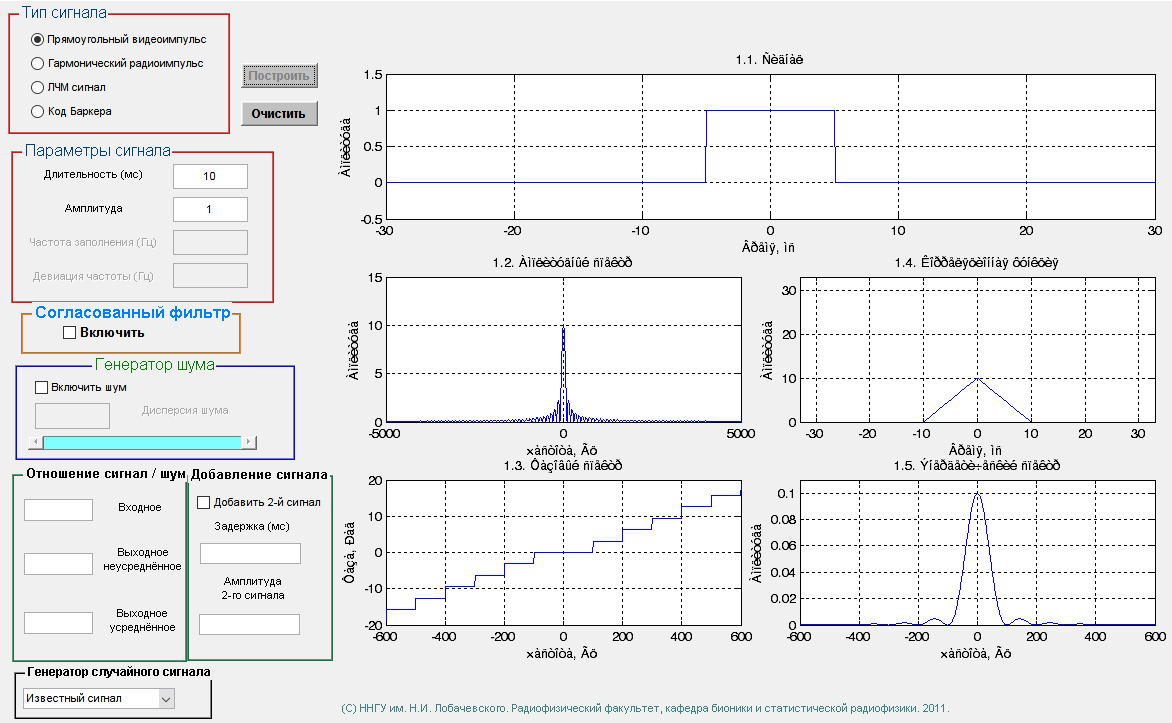
\includegraphics[width=0.9\linewidth]{imgs/t1s1_10.png}
    \caption{Приборная панель виртуального прибора. Моделируется
    прямоугольный видеоимпульс с длительность $\tau=10$ мс}
    \label{fig:task1_10}
\end{figure}
\begin{figure}[H]
    \centering
    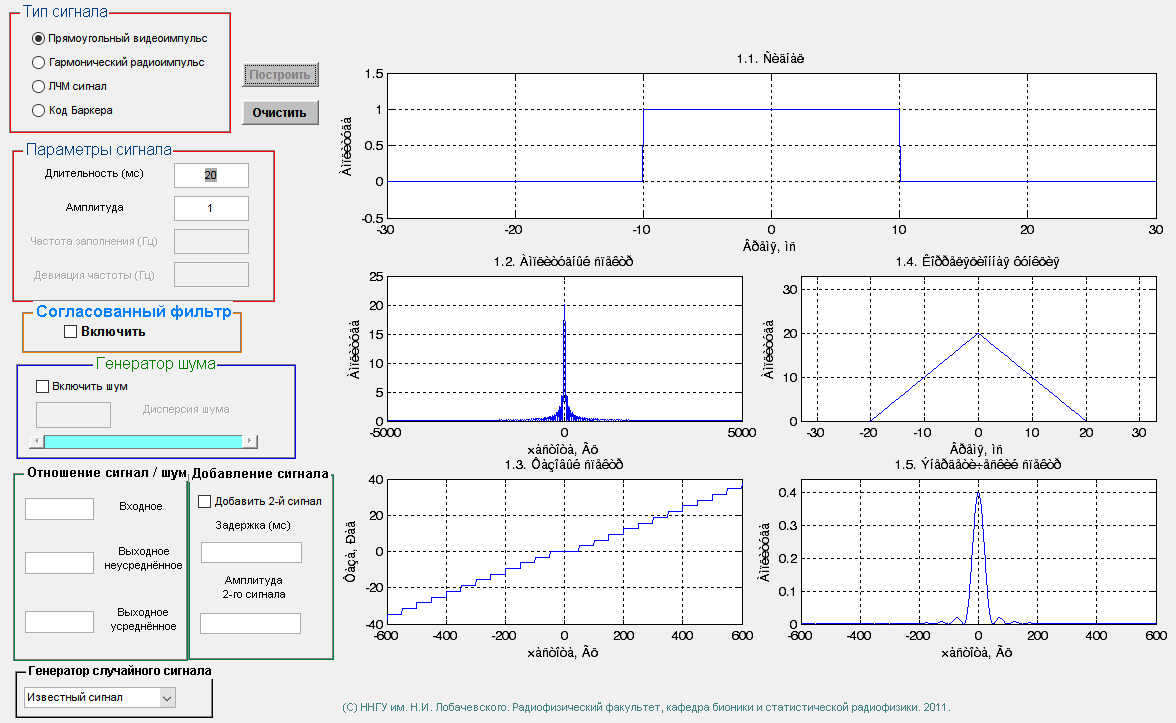
\includegraphics[width=0.9\linewidth]{imgs/t1s1_20.png}
    \caption{Приборная панель виртуального прибора. Моделируется
    прямоугольный видеоимпульс с длительность $\tau=20$ мс}
    \label{fig:task1_20}
\end{figure}


\paragraph{Оценка базы}%
\label{par:otsenka_bazy}


Найдем базу для прямоугольного импульса по следующей формуле: 
\begin{equation}
    B = T \cdot \Delta f,
    \label{eq:p:1}
\end{equation}
где $T$ - эффективная длительность, $\Delta f$ - эффективная ширина полосы спектра
сигнала(в качестве оценки берется половина ширины главного лепестка амплитудного спектра).
\begin{equation}
    B_{10ms} = 10^{-2} \cdot 100 = 1, \quad B_{20ms} = 20 \cdot 10^{-3} \cdot 50 = 1
    \label{eq:}
\end{equation}
База прямоугольного импульса равна единице, что означает что это простой сигнал. Таким образом
справедливо соотношение $\Delta f = \frac{1}{T}$. Действительно, в соответствии с этой зависимостью,
наблюдается сужение амплитудного спектра при увеличении длительности сигнала.

\paragraph{Оценка энергии}%
\label{par:otsenka_energii}


Полная энергия прямоугольного сигнала равна $A^2 \tau$  (см.
\ref{sub:theory_priamougol_nyi_impul_s} ). Поскольку, за ширину спектра мы
приняли не бесконечные пределы, а только ширину главного лепестка, то следует
пересчитать энергию. Посчитав численно интеграл для видеоимпульса с шириной
спектра $[-100, 100] \text{ Гц}$, получим, что $90.2 \%$ энергии находится в указанном
диапазоне. 


\begin{table}[H]
    \centering
    \begin{tabular}{|l|l|}
    \hline
     Диапазон & $E$ \\ \hline
     $(-\infty, \infty)$&  0.01 \\ \hline
     $(-100, 100)$&  0.00902 \\ \hline
    \end{tabular}
\end{table}

\subsubsection{Прямоугольный видеоимпульс с гармоническим заполнением}

Изучить амплитудный, фазовый и энергетический спектры. Задать
длительность импульса 10мс и 20мс, амплитуду равной 1 и частоту
заполнения 400Гц, а затем проанализировать зависимости.

\begin{figure}[H]
    \centering
    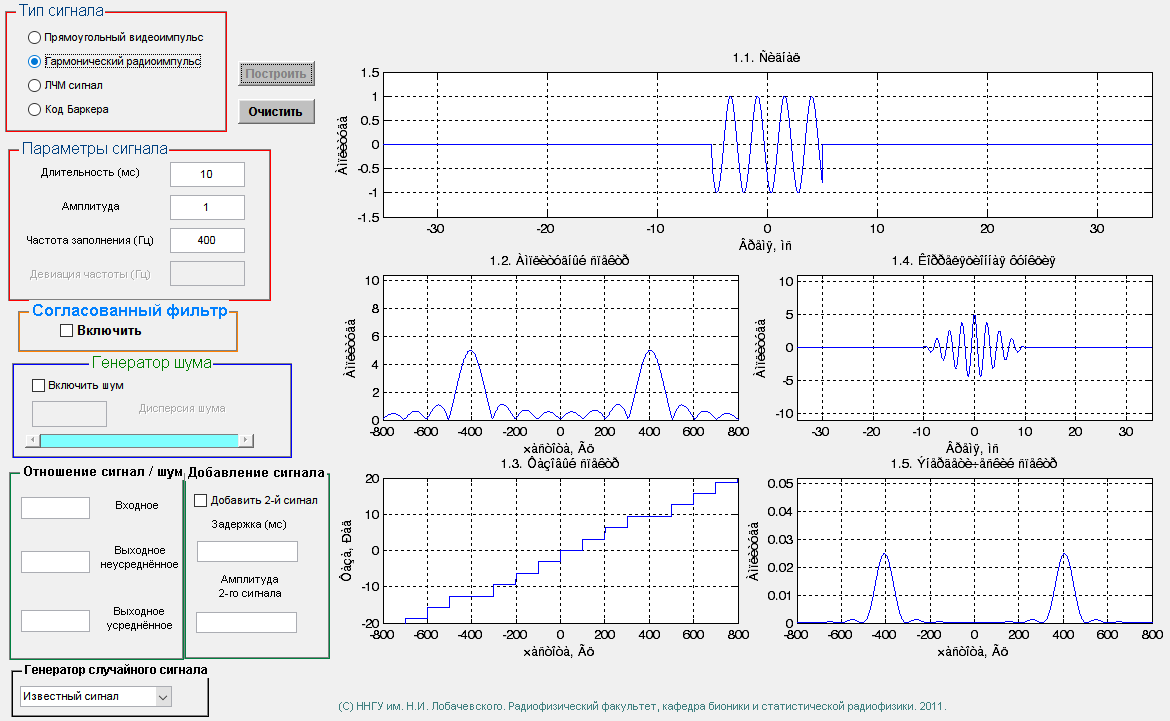
\includegraphics[width=0.9\linewidth]{imgs/t1s2_10.png}
    \caption{Приборная панель виртуального прибора. Моделируется
    прямоугольный радиоимпульс с длительность $\tau=10$ мс}
    \label{fig:task2_10}
\end{figure}
\begin{figure}[H]
    \centering
    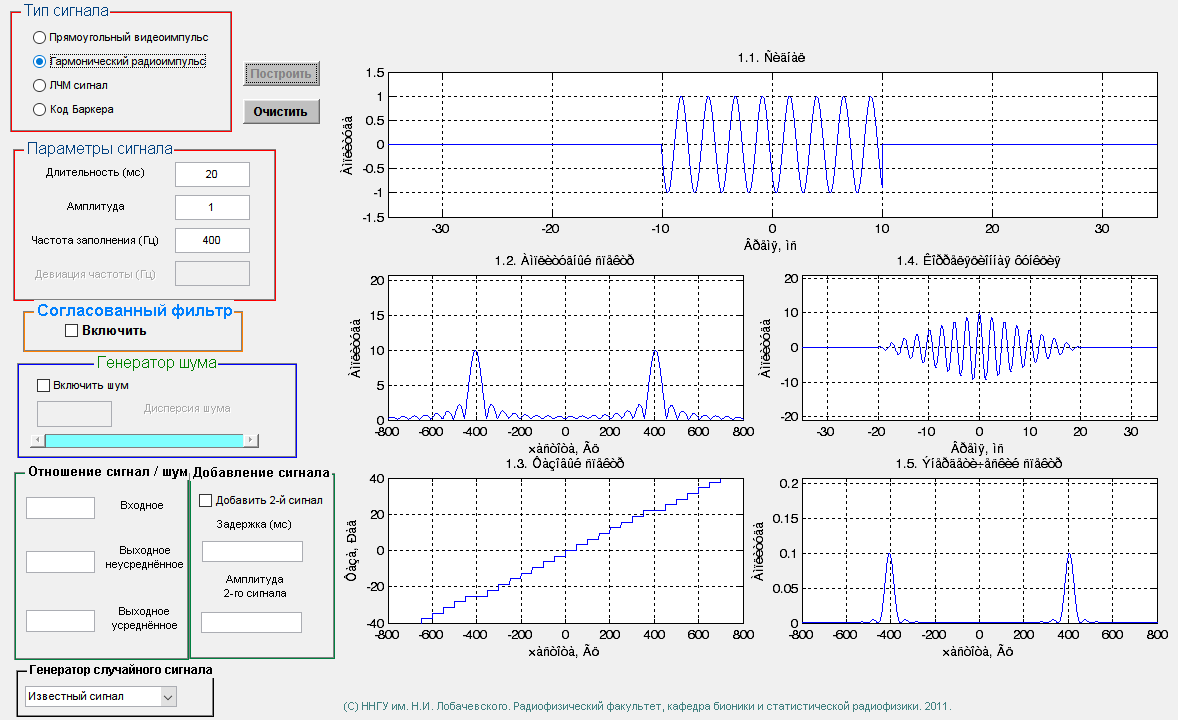
\includegraphics[width=0.9\linewidth]{imgs/t1s2_20.png}
    \caption{Приборная панель виртуального прибора. Моделируется
    прямоугольный радиоимпульс с длительность $\tau=20$ мс}
    \label{fig:task2_20}
\end{figure}

При изменении длительности импульса радиоимпульс ведет себя аналогично
видеоимпульсу, что и предсказывает теория.
\begin{equation}
    B_{10ms} = 10^{-2} \cdot 100 = 1, \quad B_{20ms} = 20 \cdot 10^{-2} \cdot 50 = 1
    \label{eq:}
\end{equation}
Значение базы - единица, означает что радиоимпульс это простой сигнал.

\subsubsection{Линейно-частотный модулированный импульс}
Получить временные реализации ЛЧМ сигнала с параметрами:
\begin{itemize}
    \item длительность 100мс, средняя частота заполнения 1000Гц,
    девиация 500Гц;
    \item длительность 100мс, средняя частота заполнения 1000Гц,
    девиация 1000Гц
    \item амплитуда 1.
\end{itemize}
\begin{figure}[H]
    \centering
    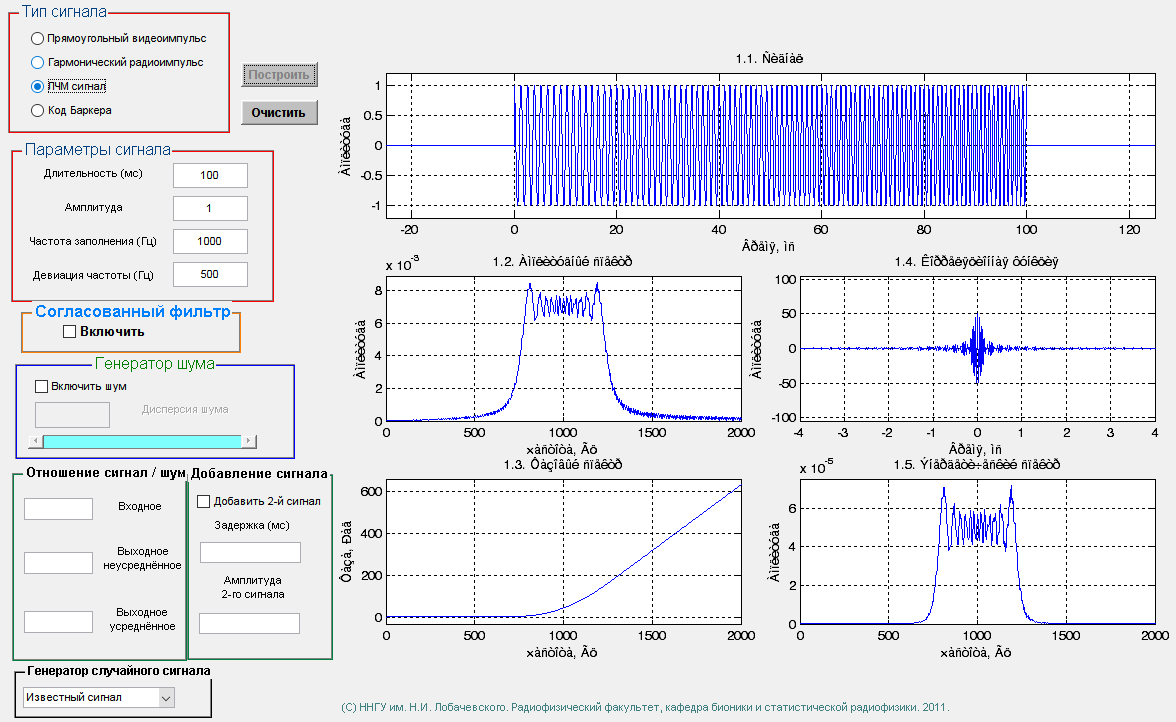
\includegraphics[width=0.9\linewidth]{imgs/t1s3_500.png}
    \caption{500 Гц}
    \label{fig:task3_500}
\end{figure}
\begin{figure}[H]
    \centering
    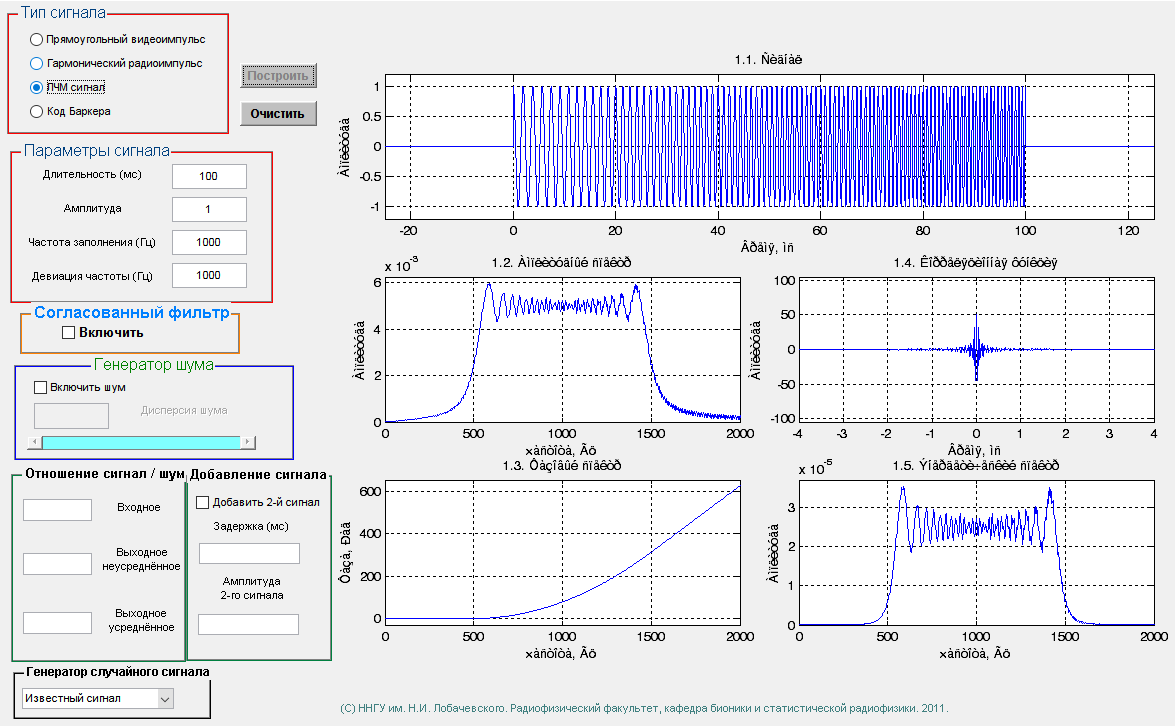
\includegraphics[width=0.9\linewidth]{imgs/t1s3_1000.png}
    \caption{1000 Гц}
    \label{fig:task3_1000}
\end{figure}

\begin{equation}
    B_{500Hz} = 100 \cdot 10^{-3} \cdot (1260-760) = 50, \quad B_{1000Hz} = 100 \cdot 10^{-3} \cdot (1500-500) = 100
    \label{eq:}
\end{equation}

\textbf{Для ЛЧМ сигнала сравнить протяженность корреляционной
функции с длительностью сигнала. Во сколько раз она меньше
длительности сигнала?}

При длительности ЛЧМ сигнала 100 мс, протяженность функции корреляции составила всего 0.4 мс, что в 250 раз меньше.

\textbf{Для ЛЧМ сигнала оценить диапазон изменения фазовых сдвигов у
гармоник сигнала в пределах полосы амплитудного спектра.
Нарисовать амплитудный спектр в приближенном виде
(аппроксимируя прямоугольником) и посмотреть, какой в этих
пределах фазовый спектр.}

Диапазон изменения фазовых сдвигов в случае девиации 500 Гц составил $\phi \in [0 - 160]$ радиан (см. рис.
\ref{fig:task3_500_phase}), в случае девиации 1000 Гц составил $\phi \in [0 - 260]$ радиан (см. рис.
\ref{fig:task3_1000_phase}).
\begin{figure}[H]
    \centering
    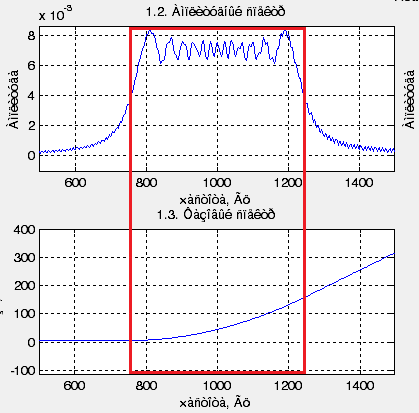
\includegraphics[width=0.5\linewidth]{imgs/t1s3_500_extra.png}
    \caption{Диапазон изменения фазовых сдвигов у гармоник сигнала, девиация 500 Гц}
    \label{fig:task3_500_phase}
\end{figure}

\begin{figure}[H]
    \centering
    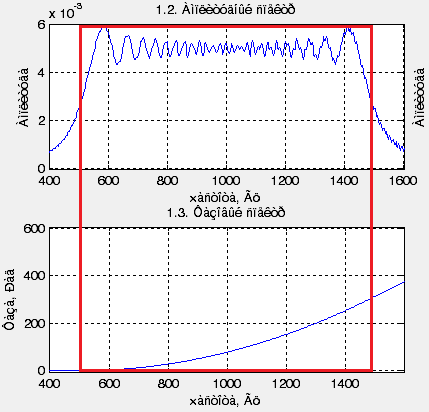
\includegraphics[width=0.5\linewidth]{imgs/t1s3_1000_extra.png}
    \caption{Диапазон изменения фазовых сдвигов у гармоник сигнала, девиация 1000 Гц}
    \label{fig:task3_1000_phase}
\end{figure}

\subsubsection{Код Баркера}
Получить реализации для кода Баркера (N=13) при длительности 13мс и
26мс
\begin{figure}[H]
    \centering
    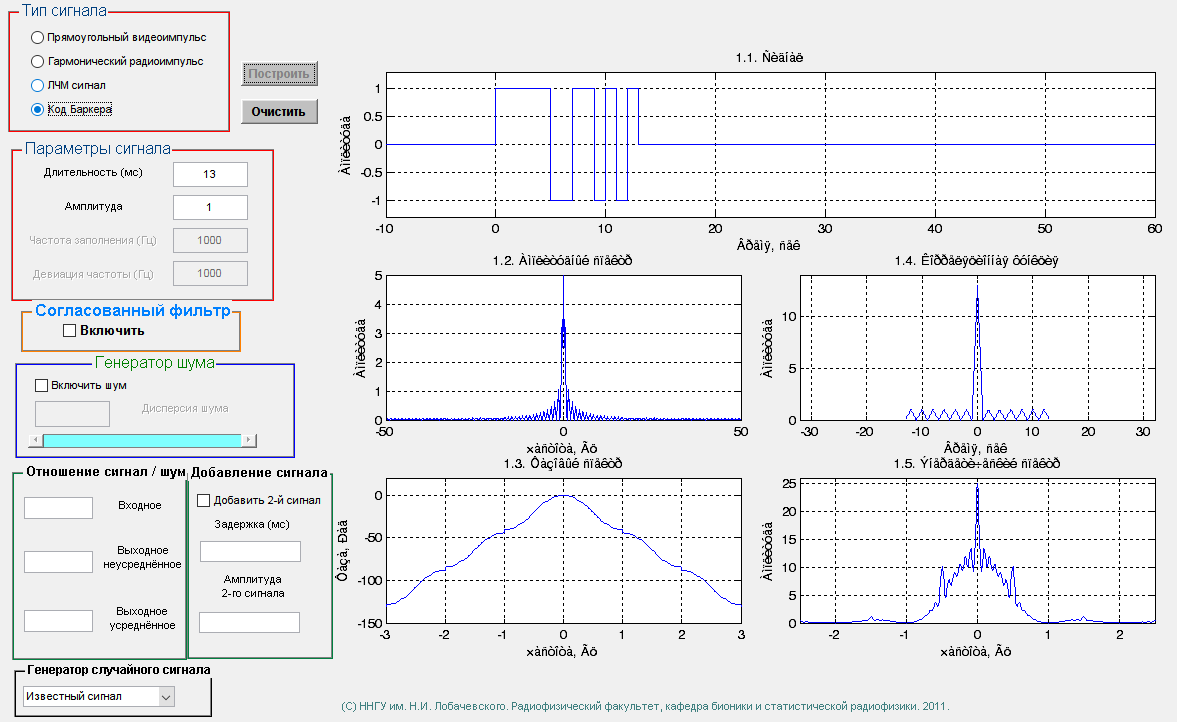
\includegraphics[width=0.9\linewidth]{imgs/t1s4_13.png}
    \caption{13 мс}
    \label{fig:task4_13}
\end{figure}

\begin{figure}[H]
    \centering
    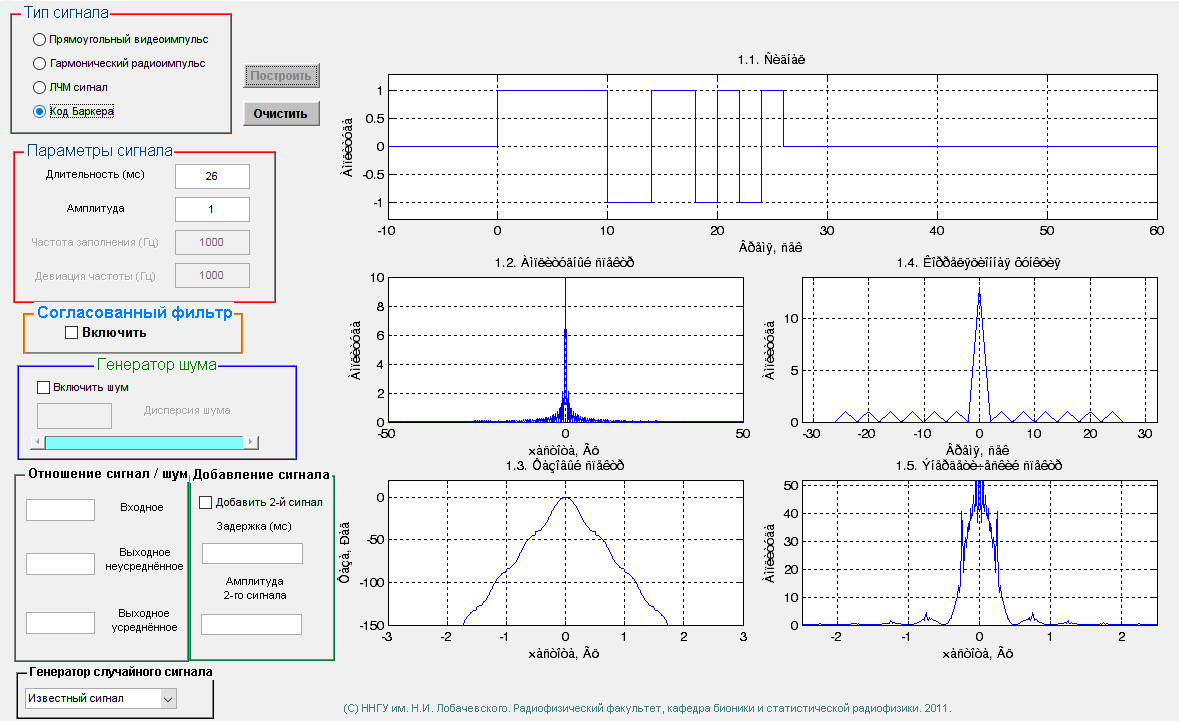
\includegraphics[width=0.9\linewidth]{imgs/t1s4_26.png}
    \caption{26 мс}
    \label{fig:task4_26}
\end{figure}

\begin{equation}
    B_{13ms} = 13 \cdot 10^{-3} \cdot 1 = 13 \cdot 10^{-3}, \quad B_{26ms} = 26 \cdot 10^{-3} \cdot 0.5 = 13 \cdot 10^{-3}
    \label{eq:}
\end{equation}

%\textbf{На что ответить в отчете:}
%\begin{enumerate}
    %\item Получить оценку энергии импульса разными способами по
    %экспериментальным данным. Сравнить результаты с
    %теоретическими.
    %\item \textbf{надо пояснения} Для всех четырех видов сигнала оценить базу,
    %используя формулу
    %$B=T \cdot \Delta f$, где T - эффективная длительность, $\Delta f$ - эффективная
    %ширина полосы спектра сигнала. За оценку ширины следует
    %принять половину расстояния между первыми нулями (ширины
    %главного лепестка).
    %\item Пояснить, как изменяется фазовый спектр сигнала, в том диапазоне
    %частот, где лежит основная энергия сигнала. Показать с помощью
    %рисунка, как происходит сложение гармонических составляющих
    %сигнала. Выделить на графиках амплитудного и энергетического
    %спектров диапазон частот, в котором лежит основная энергия
    %сигнала. Как изменяется фазовый спектр сигнала в этом диапазоне
    %частот? Почему физический амплитудный спектр имеет смысл
    %рассматривать только внутри этой полосы?
    %\item \textbf{Done, надо пояснения} Для ЛЧМ сигнала сравнить протяженность корреляционной
    %функции с длительностью сигнала. Во сколько раз она меньше
    %длительности сигнала?
    %\item \textbf{Done, надо пояснения} Для ЛЧМ сигнала оценить диапазон изменения фазовых сдвигов у
    %гармоник сигнала в пределах полосы амплитудного спектра.
    %Нарисовать амплитудный спектр в приближенном виде
    %(аппроксимируя прямоугольником) и посмотреть, какой в этих
    %пределах фазовый спектр.
    %\item Во всех примерах рассматривались изменения спектральных
    %характеристик при изменении временных зависимостей сигналов.
    %Учитывая, что для функций, сопряженных по Фурье, справедливы
    %следующие соотношения (см. Приложение)...(см методичку)
    %\item Чем определяется максимальное значение функции корреляции?
    %Рассмотреть корреляционную функцию как сигнал и найти его базу.
    %\item Сравнить изменения спектрально-корреляционных характеристик
    %при изменении длительности различных сигналов.
%\end{enumerate}



\subsection{Задание 2. Параметры согласованного фильтра и выходного сигнала}
\subsection{Задание 2. Параметры согласованного фильтра и выходного сигнала}
В этом задании изучаются характеристики согласованных фильтров,
соответствующих каждому из сигналов, рассмотренных в задании №1. Кроме
того, исследуются вид и свойства выходных сигналов. Учитывая, что при
расширении фазового спектра длительность сигнала увеличивается, а при
уменьшении до нуля – укорачивается, в данном задании необходимо
внимательно проследить за укорочением сигнала. Самый короткий и самый
большой по амплитуде он должен получиться при нулевом фазовом спектре


Рекомендации по анализу результатов эксперимента
\begin{itemize}
    \item Как коэффициент передачи по амплитуде $\abs{k(\omega)}$ фильтра и фазовые
    сдвиги $\varphi(\omega)$, вносимые фильтром в соответствующую гармонику,
    связаны с амплитудным и фазовым спектром сигнала?
    \item Как связан выходной сигнал и его амплитудный и фазовый спектр с
    характеристиками выходного сигнала? Сравнить длительности
    входного и выходного сигналов.
    \item Какой вид имеет импульсная переходная характеристика
    согласованного фильтра?
    \item Какой фазовый спектр и база выходного сигнала? 
\end{itemize}



\subsubsection{Прямоугольный видеоимпульс}
\begin{figure}[H]
    \centering
    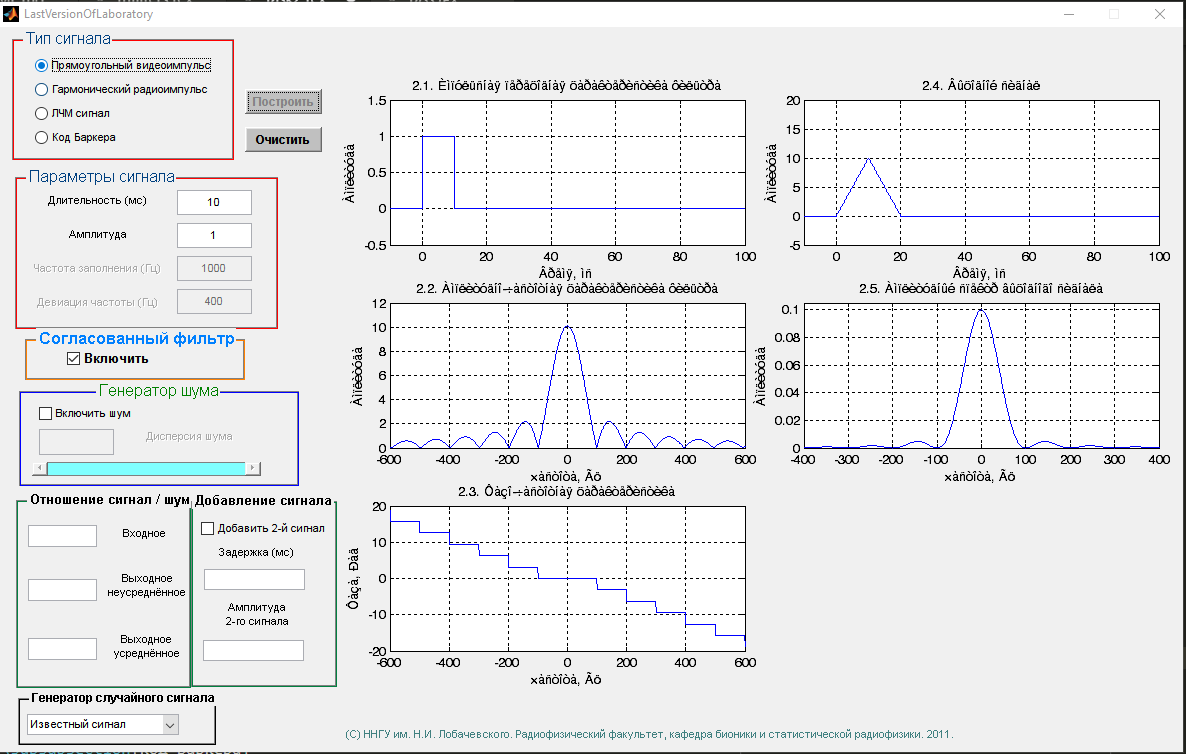
\includegraphics[width=0.9\linewidth]{imgs/task_2/t2s1_10.png}
    \caption{10 мс}
    \label{fig:task_2_1_10}
\end{figure}
\begin{figure}[H]
    \centering
    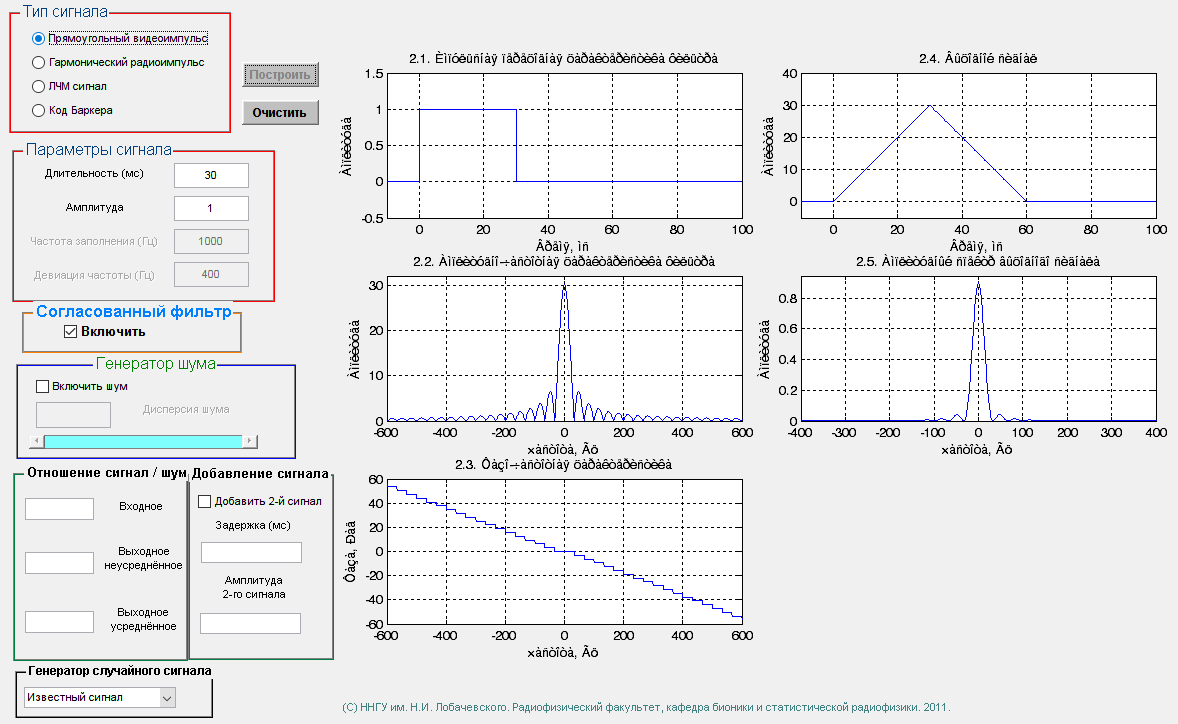
\includegraphics[width=0.9\linewidth]{imgs/task_2/t2s1_30.png}
    \caption{30 мс}
    \label{fig:task_2_1_30}
\end{figure}
АЧХ $\abs{K(i \omega)}$ и ФЧХ $\varphi (\omega)$ согласованного фильтра
\begin{equation}
    \abs{K(i \omega)} = \abs{C_0} \cdot \abs{C_m(i \omega)}, \quad
    \varphi (\omega) = -\varphi_m  -\omega t + arg(C_0),
\end{equation}
где $C_m, \varphi_m $ - амплитудный и фазовый спектры входного сигнала $m(t)$.
\begin{enumerate}
    \item 
    \item 
    \item 
    \item 
\end{enumerate}


\subsubsection{Прямоугольный видеоимпульс с гармоническим заполнением}
\begin{figure}[H]
    \centering
    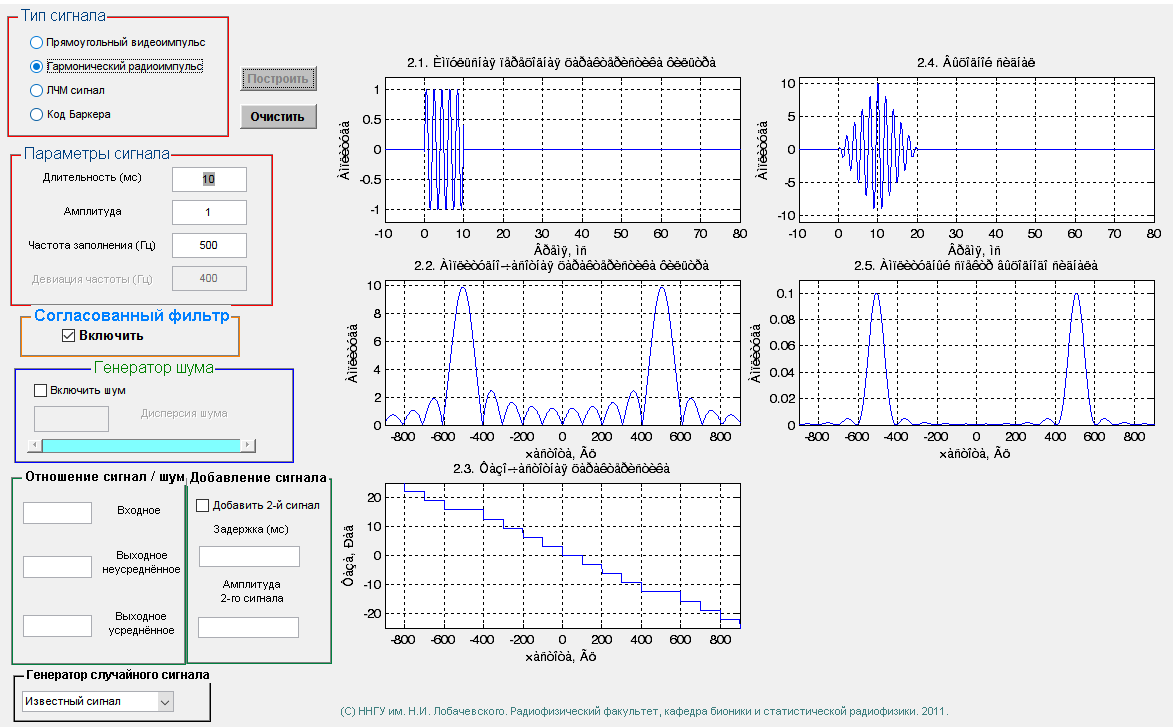
\includegraphics[width=0.9\linewidth]{imgs/task_2/t2s2_10.png}
    \caption{10 мс}
    \label{fig:task_2_2_10}
\end{figure}
\begin{figure}[H]
    \centering
    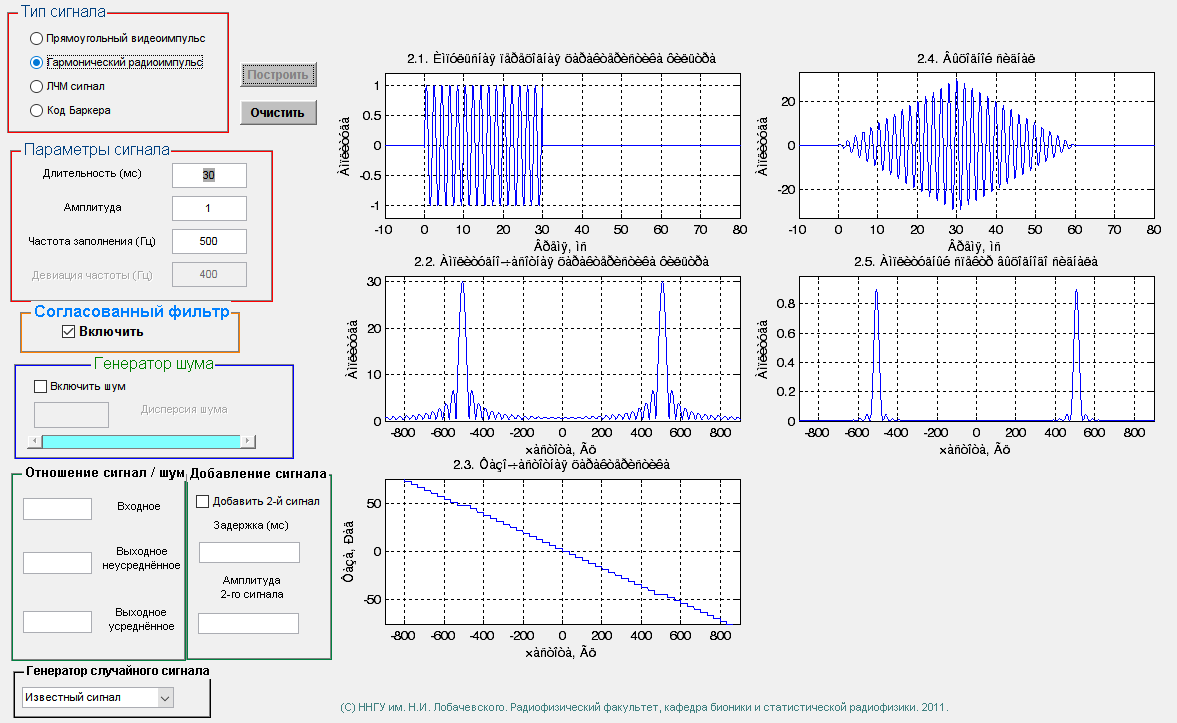
\includegraphics[width=0.9\linewidth]{imgs/task_2/t2s2_30.png}
    \caption{30 мс}
    \label{fig:task_2_2_30}
\end{figure}

\begin{enumerate}
    \item 
    \item 
    \item 
    \item 
\end{enumerate}


\subsubsection{ЛЧМ сигнал}
\begin{figure}[H]
    \centering
    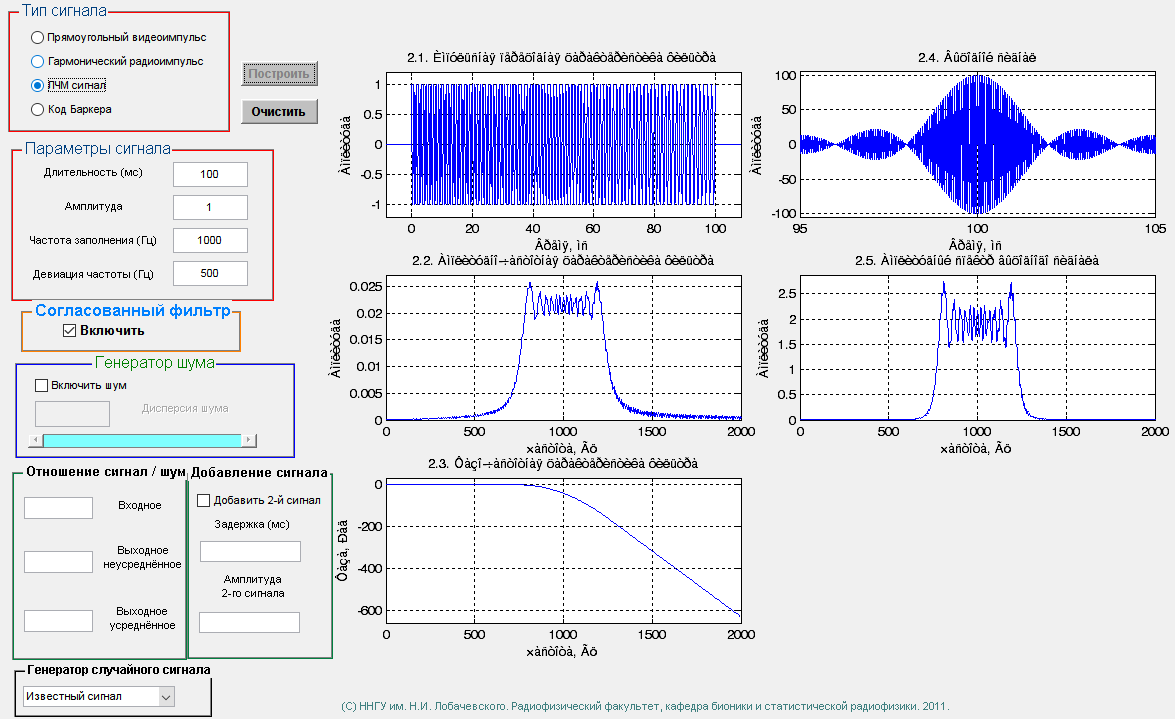
\includegraphics[width=0.9\linewidth]{imgs/task_2/t2s3_500.png}
    \caption{Девиация 500 Гц}
    \label{fig:task_2_3_500}
\end{figure}
\begin{figure}[H]
    \centering
    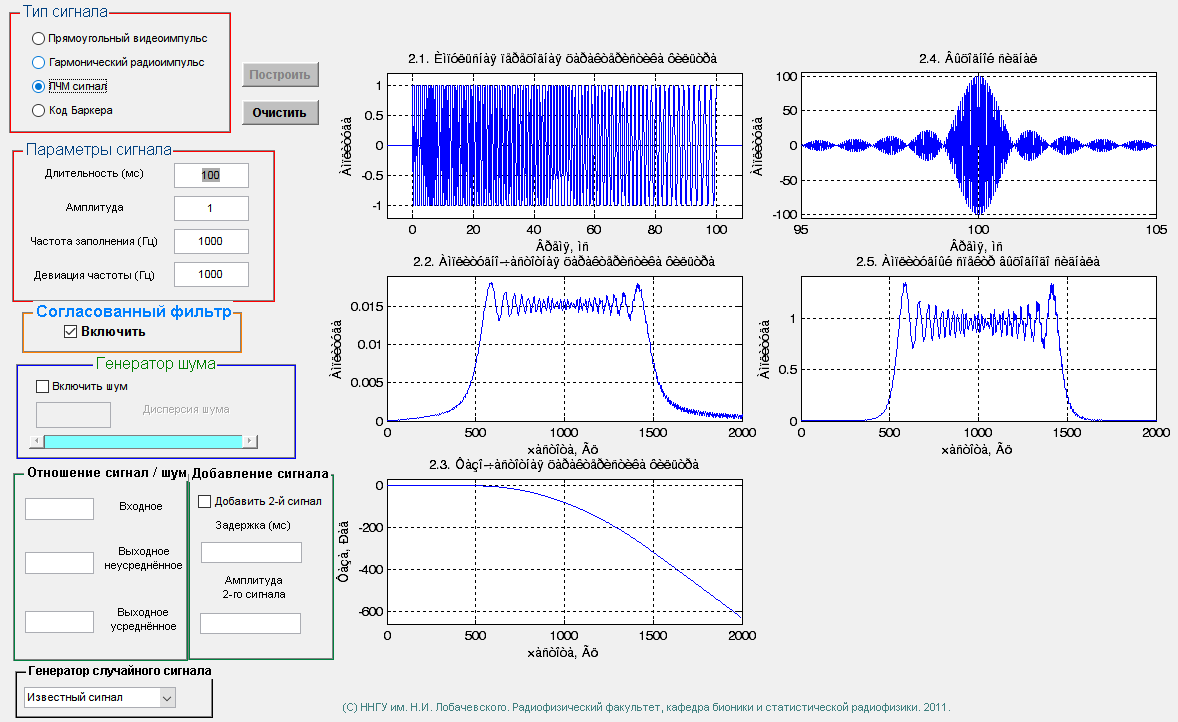
\includegraphics[width=0.9\linewidth]{imgs/task_2/t2s3_1000.png}
    \caption{Девиация 1000 Гц}
    \label{fig:task_2_3_1000}
\end{figure}

\begin{enumerate}
    \item 
    \item 
    \item 
    \item 
\end{enumerate}


\subsubsection{Код Баркера}
\begin{figure}[H]
    \centering
    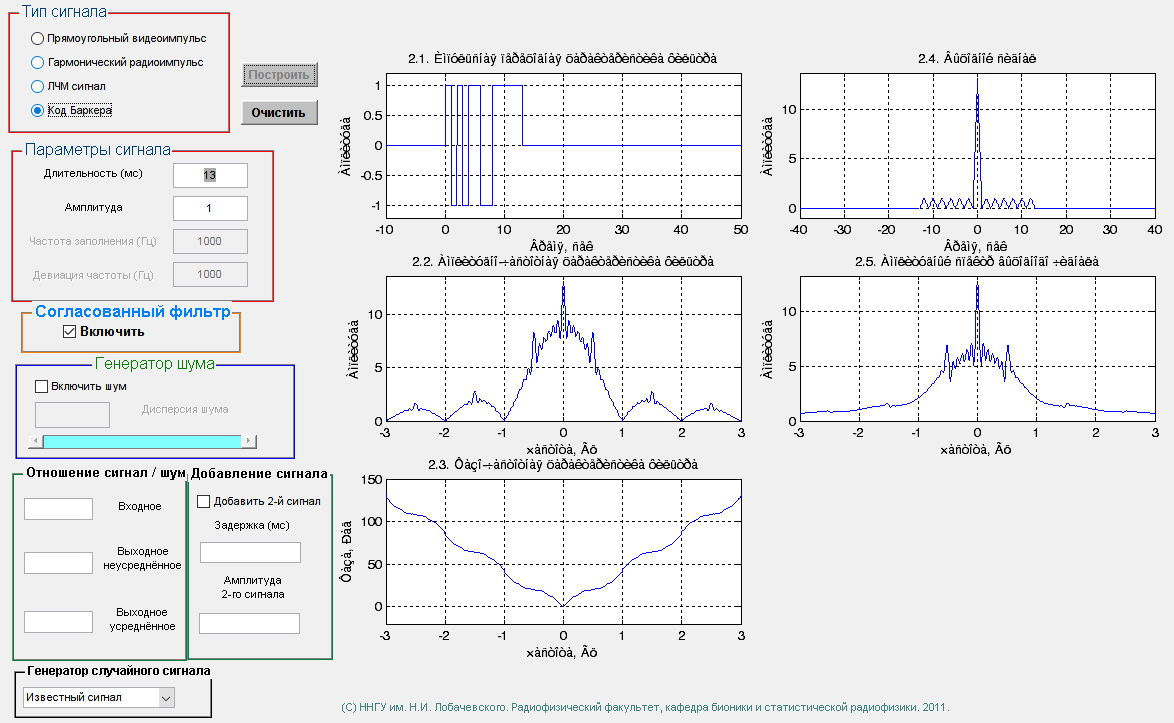
\includegraphics[width=0.9\linewidth]{imgs/task_2/t2s4_13.png}
    \caption{13 мс}
    \label{fig:task_2_4_13}
\end{figure}
\begin{figure}[H]
    \centering
    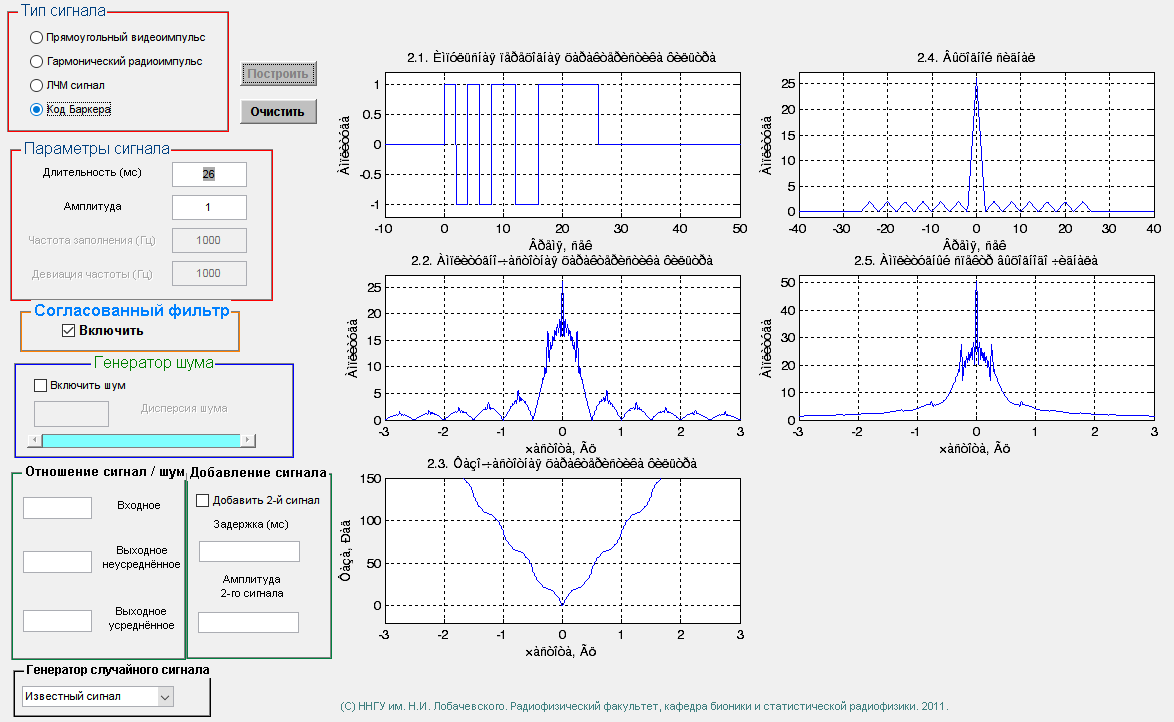
\includegraphics[width=0.9\linewidth]{imgs/task_2/t2s4_26.png}
    \caption{26 мс}
    \label{fig:task_2_4_26}
\end{figure}

\begin{enumerate}
    \item 
    \item 
    \item 
    \item 
\end{enumerate}

\subsection{Задание 3. Согласованная фильтрация линейно-частотно
модулированного сигнала}
\subsection{Согласованная фильтрация линейно-частотно
модулированного сигнала}
В этом задании на примере ЛЧМ сигнала подробно исследуются
особенности фильтрации сложных сигналов. 

%Выбрать среднюю частоту заполнения 1000Гц,
%длительность ЛЧМ сигнала менять в пределах от 10мс до 100мс
%девиацию частоты изменять от 400Гц до 1000Гц 

%Пропустить ЛАМ сигнал через согласованный фильтр. Качественно
%проанализировать, чем определяются основные параметры выходного сигнала:
%величина его максимума и степень укорочения сигнала, временное положение
%максимума. Получить и построить графики следующих зависимостей, оставляя
%среднюю частоту неизменной:


\subsubsection{Исследование зависимостей длительности выходного сигнала }%



\paragraph{Зависимость длительности выходного сигнала от длительности входного сигнала}%
\begin{figure}[H]
    \centering
    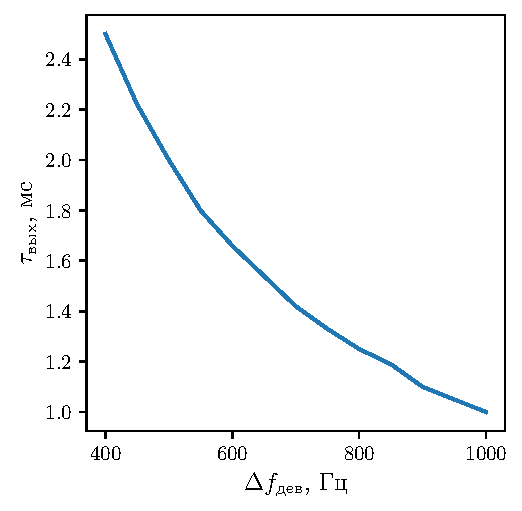
\includegraphics[width=0.6\linewidth]{imgs/task3/t3f0}
    \caption{}
    \label{fig:3.1}
\end{figure}
Зависит прямо пропорциональна, так как пиковое значение выходного сигнала
согласованного фильтра достигается не раньше, чем окончится импульсный сигнал,
поступающий на вход фильтра. Иначе невозможно накопить всю энергию входного
сигнала для формирования пика на выходе фильтра в момент времени $t_0$.
Увеличение $t_0$ сверх величины $\tau + T$ не влияет на величину максимума
выходного сигнала, а лишь сдвигает его в сторону большего запаздывания. Поэтому
имеет смысл выбирать $t_0 = \tau + T$. Тогда максимальное значение выходного
сигнала достигается точно в момент окончания входного импульса. В данном
эксперименте пиковое значение достигается в момент времени окончания входного
сигнала, так как сигнал $M(t)$ достигает максимального значения в момент $t_0$,
поскольку функция корреляции всегда имеет максимальное значение в нуле 
\begin{equation}
    \Psi^{max}_m(\tau) = \Psi_m(0)
\end{equation}
Тогда максимальное значение с точностью до постоянного множителя $C_0$
равно энергии сигнала: Формула (35)

\paragraph{Зависимость длительности выходного сигнала от девиации частоты входного сигнала}%
При увеличении девиации входного сигнала уменьшается длительность выходного
сигнала см. рис. \ref{fig:3.1}

Сжатие сигнала (его укорочение) прямо пропорционально базе сигнала. В случае
ЛЧМ сигнала база сигнала регулируется значением девиации частоты.  При
увеличении девиации уменьшается $\tau$ - характерное время выходного сигнала (см
формулу 53). При уменьшении $\tau$ увеличивается характерная ширина спектра
выходного сигнала (как следствие из Фурье-преобразования). Получаем, что при
увеличении девиации сигнала увеличивается его база.



\paragraph{Зависимость амплитуды выходного сигнала от длительности входного сигнала}%

Прямо пропорциональна (см. рис. \ref{fig:3.2}) так как при увеличении длительности
входного сигнала увеличивается суммарная энергия сигнала, и, как следствие,
увеличивается амплитуда выходного сигнала.

\begin{figure}[H]
    \centering
    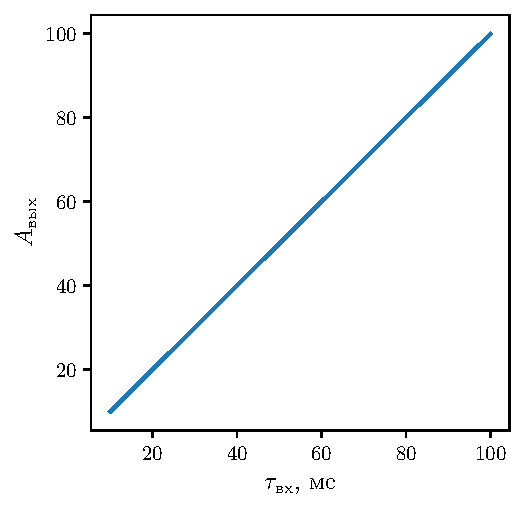
\includegraphics[width=0.6\linewidth]{imgs/task3/t3f1}
    \caption{}
    \label{fig:3.2}
\end{figure}

\paragraph{Зависимость амплитуды максимума выходного сигнала от девиации частоты входного сигнала}%
Зависимости нет, девиация частоты максимума входного сигнала не влияет на
амплитуду выходного.  Однако для других значений есть зависимость — так как при
изменении девиации входного сигнала изменяется длительность выходного сигнала
(при увеличении девиации длительность уменьшается), а значит при увеличении
девиации в любых значениях кроме максимального значения амплитуды амплитуда
выходного сигнала будет уменьшаться (при рассмотрении участка до первого нуля —
дальше значения амплитуды будут колебаться). 


\paragraph{Зависимость временного положения максимума от длительности входного сигнала}%


\begin{figure}[H]
    \centering
    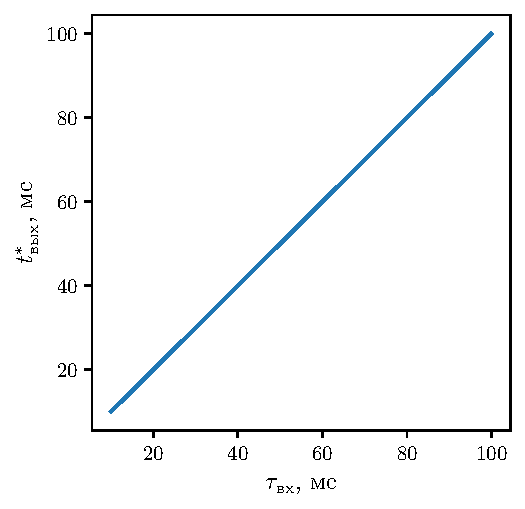
\includegraphics[width=0.6\linewidth]{imgs/task3/t3f2}
    \caption{}
    \label{fig:3.3}
\end{figure}

Прямо пропорциональна длительности входного сигнала (см. рис. \ref{fig:3.3}). Положение максимума
выходного сигнала для ЛЧМ сигнала равно времени окончания входного сигнала.

\paragraph{Зависимость временного положения максимума от девиации частоты входного сигнала}%

Не зависит. Девиация частоты не оказывает влияния на значение максимума выходного сигнала (как на его временное положение, так и на его амлитуду)



\subsection{Задание 4. Зависимость отношения сигнал/шум на выходе согласованного
фильтра от параметров входного сигнала}
В задании исследуется свойство системы с согласованным фильтром при различных
параметрах ЛЧМ сигнала: девиации частоты $\Delta f_{\text{дев}}$ и длительности
сигнала $\tau$.

\subsubsection{Однократный замер}%
\label{ssub:odnokratnyi_zamer}



\paragraph{Изменяющаяся длительность ЛЧМ сигнала}%
\label{par:izmeniaiushchaiasia_dlitel_nost_signala_tau_}

Установили девиацию частоты $\Delta f_{\text{дев}}= 700$ Гц и изменяли частоту
в пределах 10 мс -- 100 мс. 

Для одной реализации виртуальным прибором
вычислялось отношение сигнал/шум. Получившаяся зависимость приведена на рис.
\ref{fig:4.1}

\begin{figure}[h!]
    \centering
    %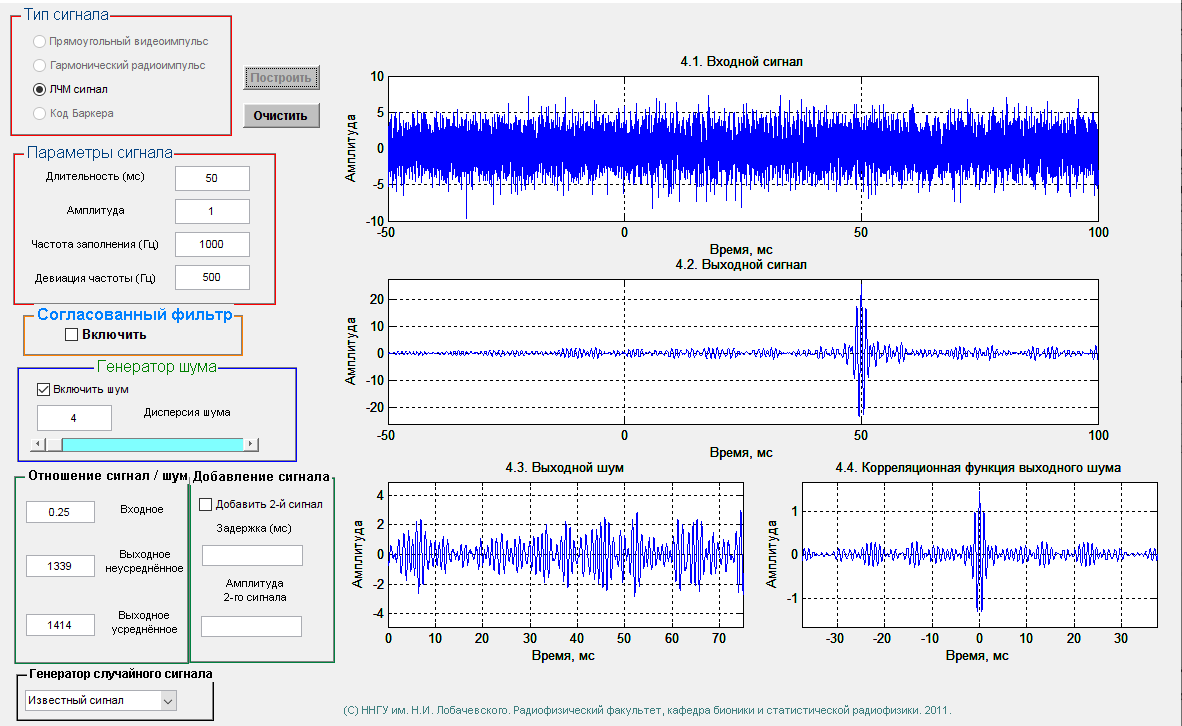
\includegraphics[width=0.6\linewidth]{imgs/t4s4_500}
    \includegraphics[width=0.6\linewidth]{example-image-a}
    \caption{}
    \label{fig:4.1}
\end{figure}

\paragraph{Изменяющаяся девиация частоты ЛЧМ сигнала}%
\label{par:izmeniaiushchaiasia_deviatsiia_chastoty_signala}
Установили длительность сигнала $\tau=50$ мс и изменяли девиацию в пределах
400 Гц - 1000 Гц.

Для одной реализации сигнала виртуальным прибором
вычислялось отношение сигнал/шум. Получившаяся зависимость приведена на рис.
\ref{fig:4.2}

\begin{figure}[h!]
    \centering
    %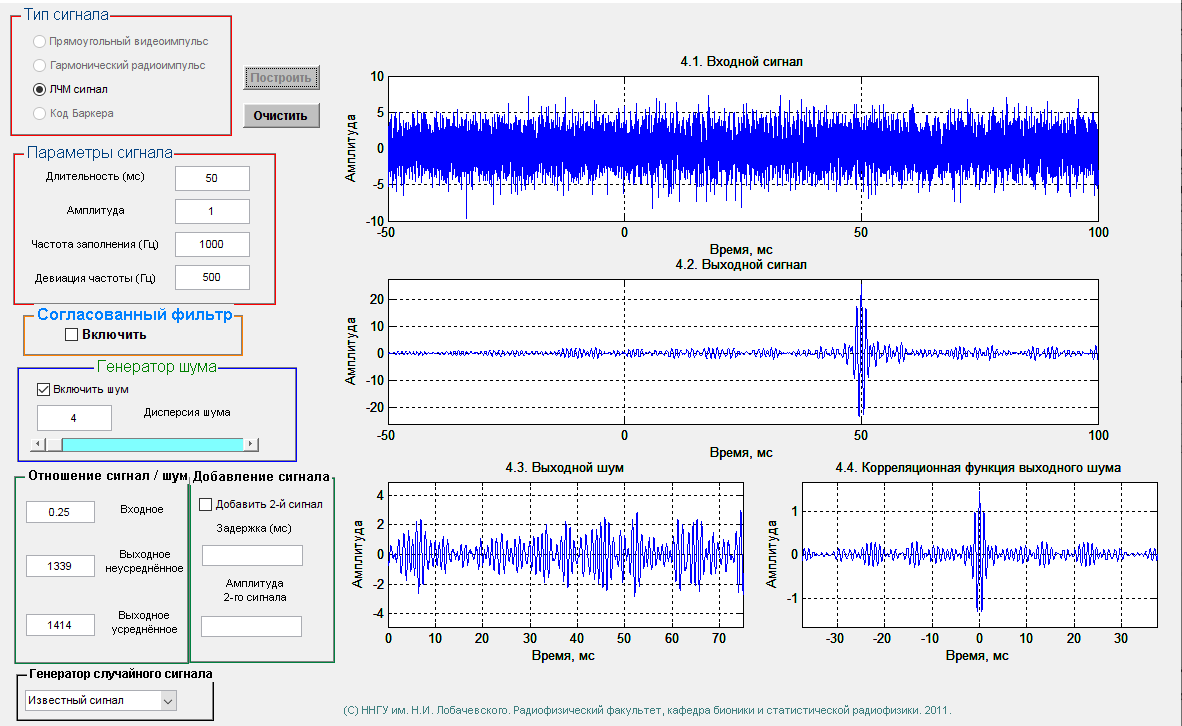
\includegraphics[width=0.6\linewidth]{imgs/t4s4_500}
    \includegraphics[width=0.6\linewidth]{example-image-a}
    \caption{Зависимость ОСШ от девиации частоты $\Delta f_{\text{дев}}$ ЛЧМ
    сигнала}
    \label{fig:4.1}
\end{figure}






\subsection{Задание 5. Разрешение во времени простых и сложных сигналов при
согласованной фильтрации.}
\subsection{Разрешение во времени простых и сложных сигналов при
согласованной фильтрации.}

Проанализируем разрешение сигналов во времени при использовании согласованного фильтра.
Качественно можно считать, что сигналы разрешены, если их максимумы
отстоят не менее, чем на величину длительности сигнала.

Отметим, что если величина временной задержки больше длительности сигнала, то входные сигналы разнесены по времени, 
и уже считаются разрешенными. Поэтому, в дальнейшем будем рассматривать задержки величиной
до длительности сигнала.

\subsubsection{Прямоугольный видеоимпульс}
Проводились измерения при значениях длительности сигналов $T = 10, 20, 40$ мс. Пример суперпозиции сигналов, а также
выход с фильтра приведены на рис. \ref{fig:task5_1_10_15}.
\begin{figure}[H]
    \centering
    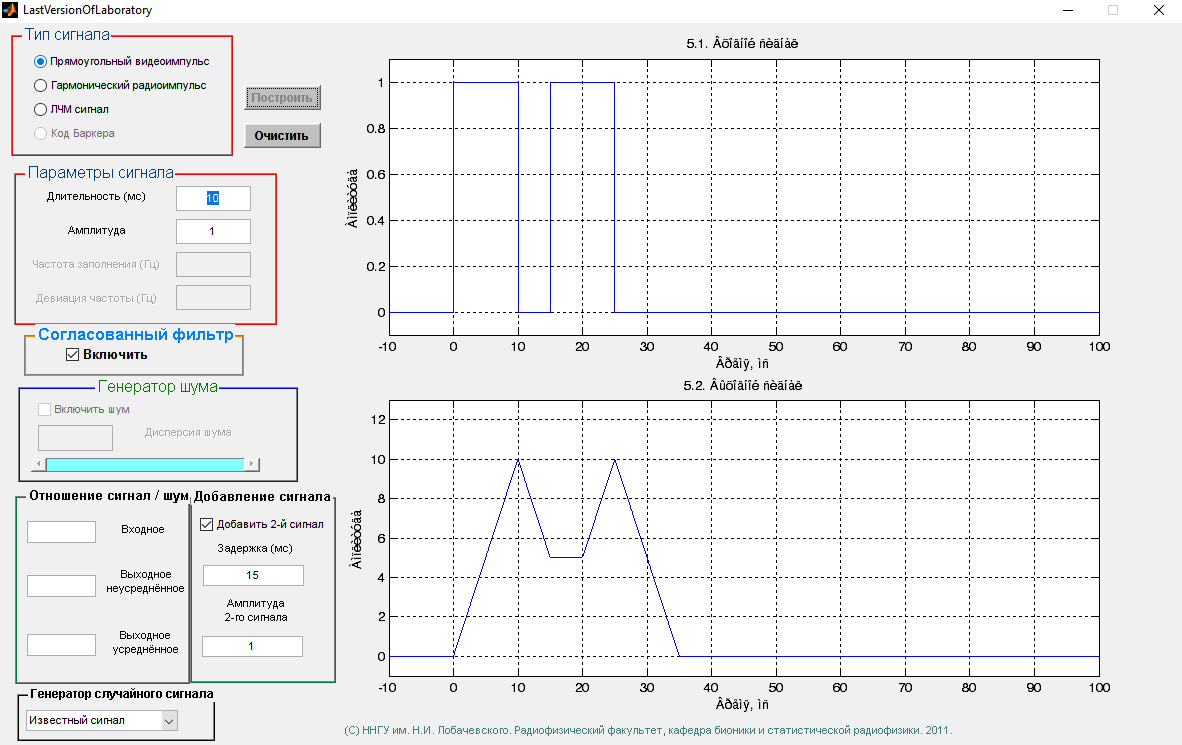
\includegraphics[width=0.7\linewidth]{imgs/task5/t5s1_dur10_del15.png}
    \caption{Прямоугольный видеоимпульс. Длительность 10 мс, задержка 15 мс}
    \label{fig:task5_1_10_15}
\end{figure}
При длительности импульса 10 мс, качественно, сигналы стали различимы при задержке в 11 мс - появились явные разделенные
пики, по которым можно различить два сигнала. Однако при задержке в 11 мс, как было скачано раньше, наступает разделение
сигналов на входе. 

Если задержка между сигналами равна длительности первого сигнала, то два входных прямоугольных видеоимпульса
сливаются в один, длительность которого становится равной 20 мс, и на входе фильтра эти сигналы не разрешены, и на
выходе согласованного фильтра наблюдается только один выходной сигнал - сигналы не разрешены.

Использование согласованной фильтрации не позволяет разрешить два прямоугольных видеоимпульса подданных неразрешенными на вход фильтра. 



\subsubsection{ЛЧМ сигнал}
Далее исследовался ЛЧМ сигнал с частотой заполнения $f=3000$ Гц, девиацией $\Delta f = 200, 400, 800$ Гц, одинаковыми амплитудами, и
длительностью $T=10, 20, 40$ мс. ЛЧМ сигналы это сложные сигналы, чья база $B$ много больше единицы: $B = T \cdot \Delta f \in [2,32]$
\begin{figure}[H]
    \centering
    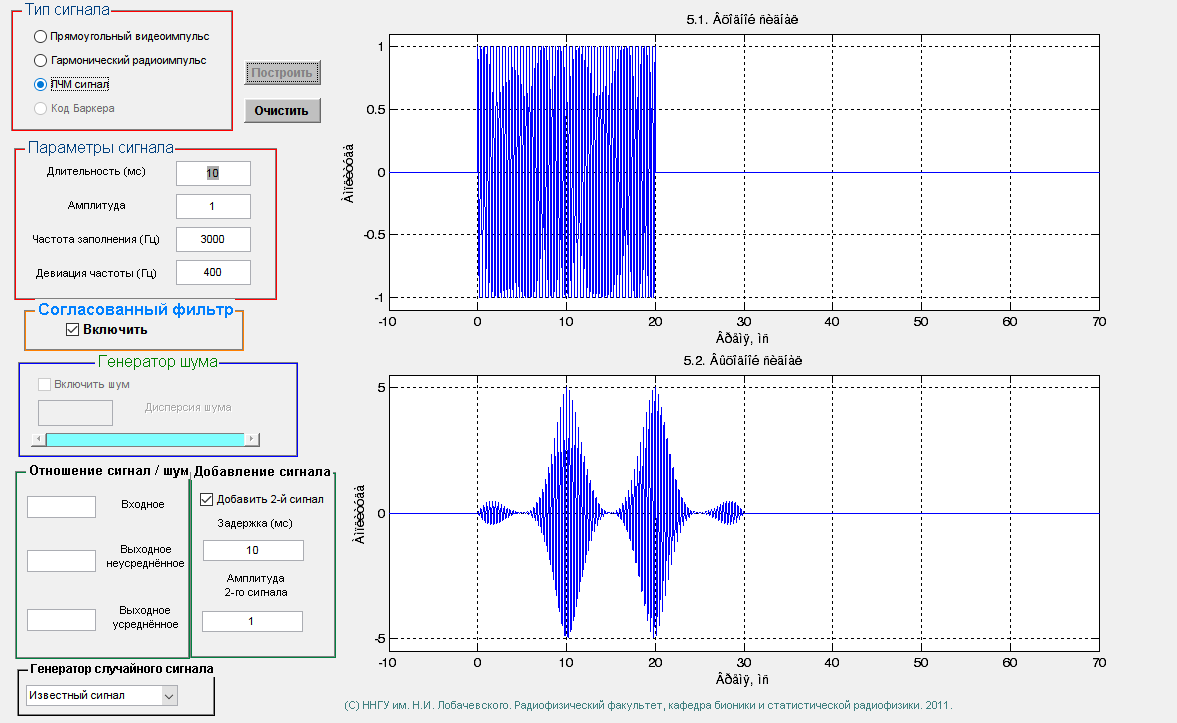
\includegraphics[width=0.6\linewidth]{imgs/task5/lfm_dev400/t5s21_dur10_del10_dev400.png}
    \caption{ЛЧМ сигнал, $T=10$ мс, $\Delta f=400$ Гц, $\Delta t=10$ мс}
    \label{fig:t5s21_dur10_del10_dev400}
\end{figure}

Рассмотрим сигналы с одинаковой амплитудой и длительностью.
На рис. \ref{fig:t5s21_dur10_del10_dev400} приведены осциллограммы входного и выходного сигнала, длительностью
$T=10$ мс, $\Delta f=400$ Гц, значение задержки $\Delta t = 10$ мс. На входе сигналы не разрешены - они сливаются в один
сигнал длительностью 20 мс, однако на выходе согласованного фильтра наблюдается два разнесенных по времени пика.

Так происходит, потому  что эффеткивная длительность сигнала уменьшается в $B$ раз при прохождении согласованного фильтра. Таким образом,
эффективная длительность каждого сигнала на выходе:
\begin{equation}
    T_{eff} = \frac{T}{B} = \frac{1}{\Delta f}=\frac{10}{4} = 2.5 \text{мс}
    \label{eq:effective_dur}
\end{equation}

В случае, когда задержка меньше длительности, например $\Delta t = 5$ мс, на входе сигналы перекрываются
(см. рис. \ref{fig:t5s21_dur10_del5_dev400}). При этом на выходе согласованного фильтра все также наблюдаются два
отчетливо разнесенных отклика.
\begin{figure}[H]
    \centering
    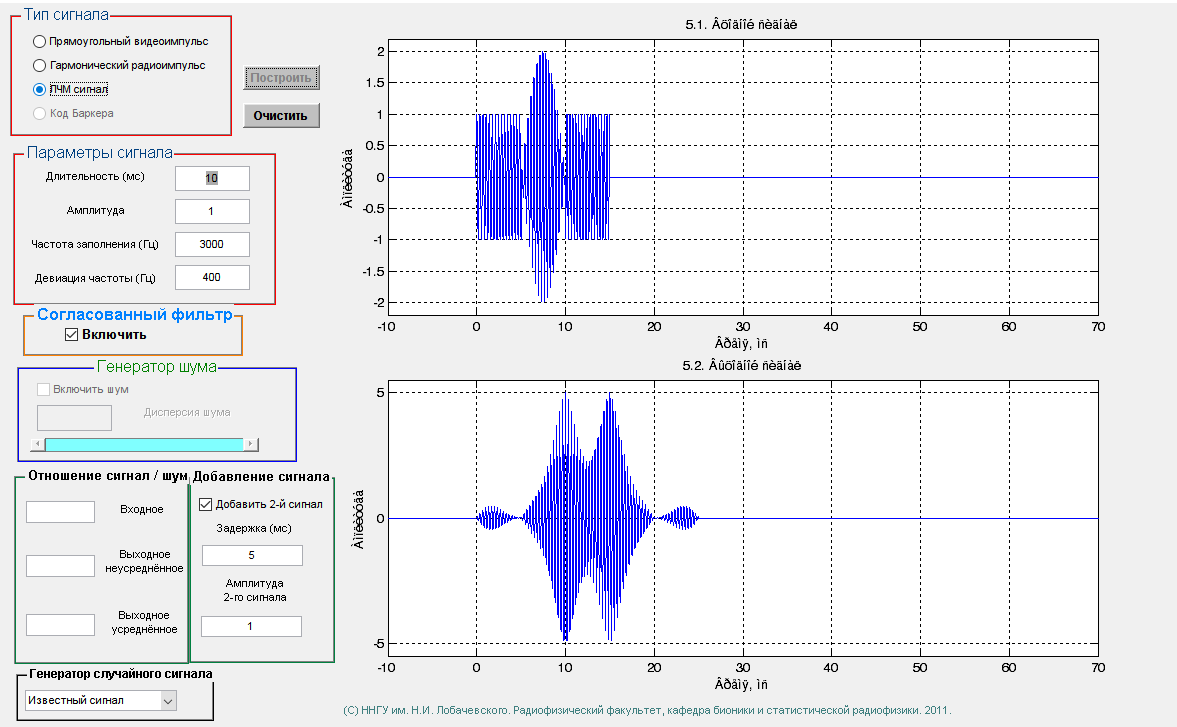
\includegraphics[width=0.6\linewidth]{imgs/task5/lfm_dev400/t5s21_dur10_del5_dev400.png}
    \caption{ЛЧМ сигнал, $T=10$ мс, $\Delta f=400$ Гц, $\Delta t=5$ мс}
    \label{fig:t5s21_dur10_del5_dev400}
\end{figure}

Для сигнала в $T=10$ мс, $\Delta f=400$ Гц, значение задержки $\Delta t$, при котором становятся различимы сигналы,
составляет $\Delta t=6$ мс.

Далее варьировались параметры сигналов и определялось минимальное значение временной задержки сигналов.
По результатам измерений была составлена следующая таблица, в которой указаны пороговые значения задержки в мс, при
которых сигналы становились различимыми:
\begin{table}[H]
    \centering
    \begin{tabular}{|x{2.0cm}|l|l|l|}
    \hline
    \diag{.1em}{2.0cm}{$\Delta f$, Гц }{T,мс}  & 10 & 20 & 30 \\ \hline
    200 &  6  &  6  &  7  \\ \hline
    400 &  3  &  3.05  &  3.05  \\ \hline
    800 &  1.2  &  1.1  &  1.1  \\
    \hline 
    \end{tabular}
\end{table}
Из полученных данных видно, что увеличение длительности сигнала слабо практически не влияет на разрешающую способность,
в то время как величина девиации напрямую влияет на разрешающую способность - эффективная длительность сигнала на выходе $T_{eff} =
\frac{1}{\Delta f}$. Укорачивая длительность сигналов, они разносятся на выходе, повышая разрешающую способность.

Видно преимущество сложных сигналов - даже слившиеся или перектрытые сигналы можно разрешить,
используя согласованный фильтр.

Также рассмотрим сигналы с разной амплитудой. Пусть амплитуда задержанного сигнала меньше основного в $\sim 6$ раз.
Длительность $T=10$ мс, $\Delta f=400$ Гц, значение задержки $\Delta t = 10$ мс (см. рис. \ref{fig:t5s21_dur10_del10_dev400_amp6}).
\begin{figure}[H]
    \centering
    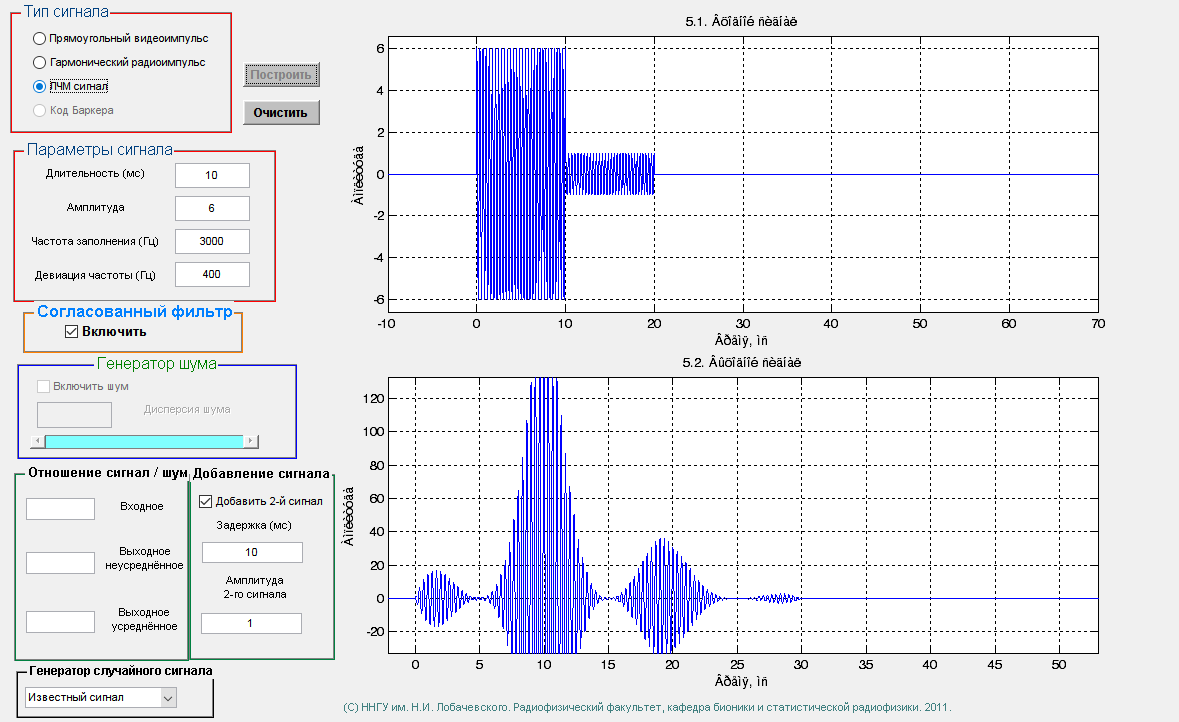
\includegraphics[width=0.6\linewidth]{imgs/task5/lfm_dev400/6amp/t5s21_dur10_del10_dev400_amp6.png}
    \caption{ЛЧМ сигнал, $T=10$ мс, $\Delta f=400$ Гц, $\Delta t=10$ мс, $A_1 = 6A_2$}
    \label{fig:t5s21_dur10_del10_dev400_amp6}
\end{figure}
На выходе фильтра наблюдается два отклика, разнесенные по времени. Таким образом, сигналы разрешены и на входе (по
амплитуде), и на выходе (по времени). Однако стоит отметить, что в данной ситуации отклик второго испульса накладывается
на побочный лепесток первичного импульса, и возможна ситуация, при которой сигналы будет невозможно разрешить.

\paragraph{Вывод}
Используя сложные сигналы, можно обеспечить необходимую разрешающую способность, поскольку проходя через согласованный
фильтр, эффективная длительсноть сигнала сокращается в $B$ раз, что бессмысленно в случае с простыми сигналами, которые
невозможно различить при задержке меньше длительности.


\subsection{Задание 6. Различение сигналов.}
\subsection{Задание 6. Различение сигналов.}


\section{Вывод}


\newpage
\section{Дополнение}
\textit{Здесь приведены некоторые вопросы, которые разбирались на сдаче отчета}

\end{document}
